
Das Usenet ist noch immer eine umfangreiche Quelle f�r Informationen zu aktuellen Themen.\\

Dabei geht es nicht immer um die im Artikel ver�ffentlichten Informationen. Auch �ber den Absender l��t sich viel herausfinden. Die folgenden Hinweise sollen eine Recherche zur Erstellung eines Pers�nlichkeitsprofiles erschweren:

\begin{itemize}
 \item Um eine langfristige Speicherung der Postings zu verhindern sollte ein zus�tzlicher Header ins Posting eingef�gt werden: \textit{X-No-Archive: yes}
\item Es sollte ein News-Server genutzt werden, der SSL-Verschl�sselung bietet und m�glichst wenig �ber den Absender preisgibt.
\item Man k�nnte seine Identit�t regelm��ig wechseln, sofern keine besondere Reputation mit einer bestimmten Identit�t verbunden ist.
\item Mail2News-Gateways k�nnen zum Versenden des Postings genutzt werden. Das Posting wird per E-Mail an das Gateway gesendet, welches es dann an den Newsserver �bermittelt. In der Regel �bernehmen Mail2News-Gateways die Absender- und IP-Adresse. Eine Liste gut erreichbarer Gateways:
\begin{itemize}
 \item mail2news (at) m2n.mixmin.net
\item mail2news (at) dizum.com
\item mail2news (at) bananasplit.info
\item mail2news (at) reece.net.au
\end{itemize}

\item Remailer bieten die M�glichkeit, anonyme Beitr�ge zu ver�ffentlichen. Das Posting wird dabei als anonyme E-Mail an ein Mail2News-Gateway gesendet.\\

Da anonymes Posten insbesondere in deutschen News-Gruppen nicht gern gesehen wird, sollte man gut �berlegen, ob es wirklich n�tig ist. Ein Pseudonym reicht meistens auch.\\

Wer die n�tige Installation der Software scheut, kann ein Webinterface nutzen unter:
\begin{itemize}
 \item \href{https://www.awxcnx.de/anon-news.htm}{https://www.awxcnx.de/anon-news.htm}
 \item \href{https://www.cotse.net/cgi-bin/mixnews.cgi}{https://www.cotse.net/cgi-bin/mixnews.cgi}
 \item \href{https://www.bananasplit.info/cgi-bin/anon.cgi}{https://www.bananasplit.info/cgi-bin/anon.cgi}
\end{itemize}


\end{itemize}

\section{News-Server}
Der Server news.mixmin.net bietet SSL-Verschl�sselung f�r den lesenden Zugriff und einen ebenfalls TLS-verschl�sselten SMTP-Zugang f�r das Senden von News-Beitr�gen.\\

Server-Einstellungen:
\begin{verbatim}
   News-Server: news.mixmin.net
   Port:        563 (SSL-verschl�sselt)

   SMTP-Server: news.mixmin.net
   Port:        25 (TLS-verschl�sselt)
\end{verbatim}

news.mixmin.net verwendet ein SSL-Zertifikat, welches von CAcert.org signiert wurde. Standartm��ig wird diese CA nur von wenigen Newsreadern aktzeptiert. Das Root-Zertifikat von CAcert.org ist von \href{http://www.cacert.org}{http://www.cacert.org} zu holen und zu importieren.\\

Die Nutzung von TOR als anonymisierender Proxy ist nach unseren Erfahrungen problemlos m�glich.
\newpage
\section{Thunderbird konfigurieren}
\begin{enumerate}
 \item Anlegen eines neuen SMPT-Servers. Diese Server findet man im Dialog \textit{Konten...} ganz unten. Der bereits konfigurierte Standard-Server tut es aber auch (und protokolliert jedes Posting).
\item Erstellen und Einrichten eines News-Kontos. Dabei ist auch der SMTP-Server auszuw�hlen.
\item Hinzuf�gen des Headers \textit{X-No-Archive: yes} f�r das News-Konto.\\

Im Einstellungs-Dialog von Thunderbird findet man in der Sektion \textit{Erweitert} den Reiter \textit{Allgemein}. Ein Klick auf den Button \textit{Konfiguration bearbeiten} �ffnet eine Liste aller Optionen.\\

\begin{figure}[htb]
\begin{center}
 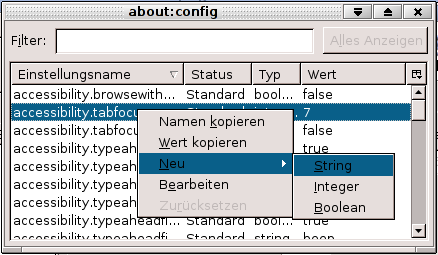
\includegraphics[scale=0.65]{../screenshots/thunderbird_uafake.png}
\caption{Neue Config-Variable anlegen}
\label{abb:thunderbird_allconfig}
\end{center}
\end{figure}

Hier f�gt man zwei neue String-Variablen mit folgenden Werten ein (\textbf{N} entspricht dabei der id-Nummer des News-Kontos):\\

% use packages: array
\begin{tabular}{ll}
mail.identity.id\textbf{N}.headers &  archive\\ 
mail.identity.id\textbf{N}.header.archive & X-No-Archive: yes
\end{tabular}
\item Abonnieren der News-Gruppen.
\end{enumerate}

